\section{Introduction}

\subsection{What is a robot?}

A robot is a \textbf{mechatronic system} designed to interact with its environment. It typically includes:
\begin{itemize}
  \item An \textbf{actuation system} to generate motion.
  \item A \textbf{sensing system} to acquire and process information about itself and the external world.
  \item A \textbf{control or AI system} to program and control its behavior.
\end{itemize}

A robot is therefore a \textbf{complex system} that embeds various technologies from mechanics, electronics, computer science, and artificial intelligence.

\begin{figure}[H]
  \centering
  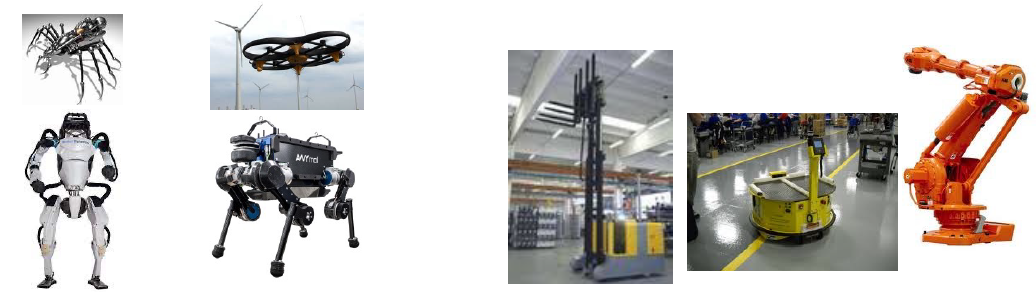
\includegraphics[width=\linewidth]{imgs/introduction_what_is_a_robot.png}
  \caption{Examples of different types of robots.}
\end{figure}

\hfill

\subsection{Robotics applications}

The first \textit{modern} robots were developed in the 1950s to support the teleoperation of radioactive materials and for prosthetic applications.

Robots began appearing in industrial environments in the 1970s, particularly in companies like General Motors. They were mainly employed for:
\begin{itemize}
  \item Welding
  \item Assembly
  \item Other repetitive and hazardous operations
\end{itemize}

Nowadays, robots are widely used in many other domains:
\begin{itemize}
  \item Medicine
  \item Space
  \item Military
  \item Entertainment
  \item \dots
\end{itemize}

\hfill

\subsection{Industrial Robotic Arms}

Industrial robotic arms are widely used in manufacturing and production lines. They are designed to perform specific, repetitive tasks with high precision and speed.

Typical applications include:
\begin{itemize}
  \item Mechanics
  \item Painting
  \item Placements
  \item Measurement control
\end{itemize}

\hfill
\begin{figure}[H]
  \centering
  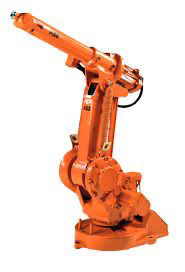
\includegraphics[width=0.2\linewidth]{imgs/industrial_robot_arm.png}
  \caption{Examples of different types of robots.}
\end{figure}

\hfill

\subsection{Industrial robotics}

In traditional industrial applications, robotic arms are employed for tasks that require:
\begin{itemize}
  \item High precision
  \item High repeatability
  \item High payload capacity
\end{itemize}

To guarantee safety, industrial robots are typically enclosed within physical barriers such as fences, preventing human access during operation.

Moreover, these robots are usually painted in bright colors to alert and warn operators of potential hazards in the workspace.

\hfill

\subsection{Advanced perception}

Advanced perception is a key component in modern robotics, especially within industrial robotic cells. Among all sensors, vision sensors are the most frequently used.

The main types of vision sensors include:
\begin{itemize}
  \item \textbf{Cameras}, which capture 2D images and video.
  \item \textbf{3D vision sensors}, which provide depth perception and spatial understanding.
\end{itemize}

These tools are essential for enabling robots to detect, recognize, and interact with objects in their environment.

\begin{figure}[H]
    \centering
    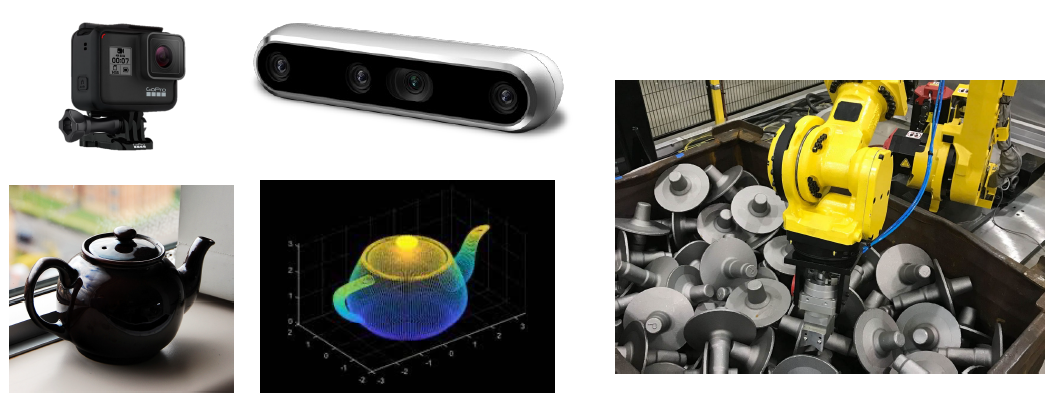
\includegraphics[width=\linewidth]{imgs/advanced_perception_sensors.png}
    \caption{Advanced perception sensors examples}
\end{figure}

\hfill

\subsection{Collaborative Robotics}

Collaborative robotics refers to systems where humans and robots operate together in a shared workspace.

Key features:
\begin{itemize}
  \item Human(s) and robots collaborate in the same area.
  \item No physical barriers are present between them.
\end{itemize}

\hfill
\begin{figure}[H]
    \centering
    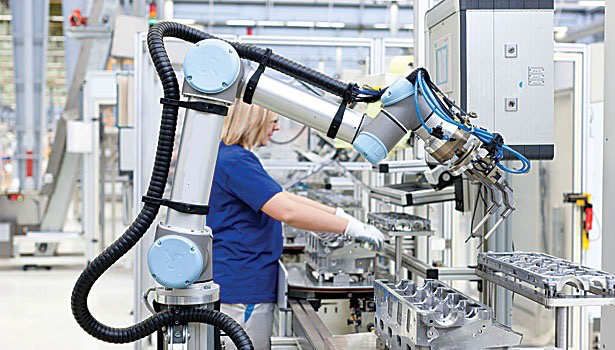
\includegraphics[width=0.6\linewidth]{imgs/collaborative_robotics_example.png}
    \caption{Collaborative robotics example}
\end{figure}

\hfill

\subsection{Collaboration}

There are various types of human-robot interaction, depending on the goal and the nature of the task.

The main distinctions are based on:
\begin{itemize}
  \item The proximity between the human and the robot (e.g., wearable, in-hand, arm's length, or out of reach).
  \item The frequency and level of interaction, which relate to the robot's agency.
\end{itemize}

These categories range from wearable robotics and teleoperated devices to highly interactive systems such as cooperative, collaborative, and supportive robots.

\begin{figure}[H]
  \centering
  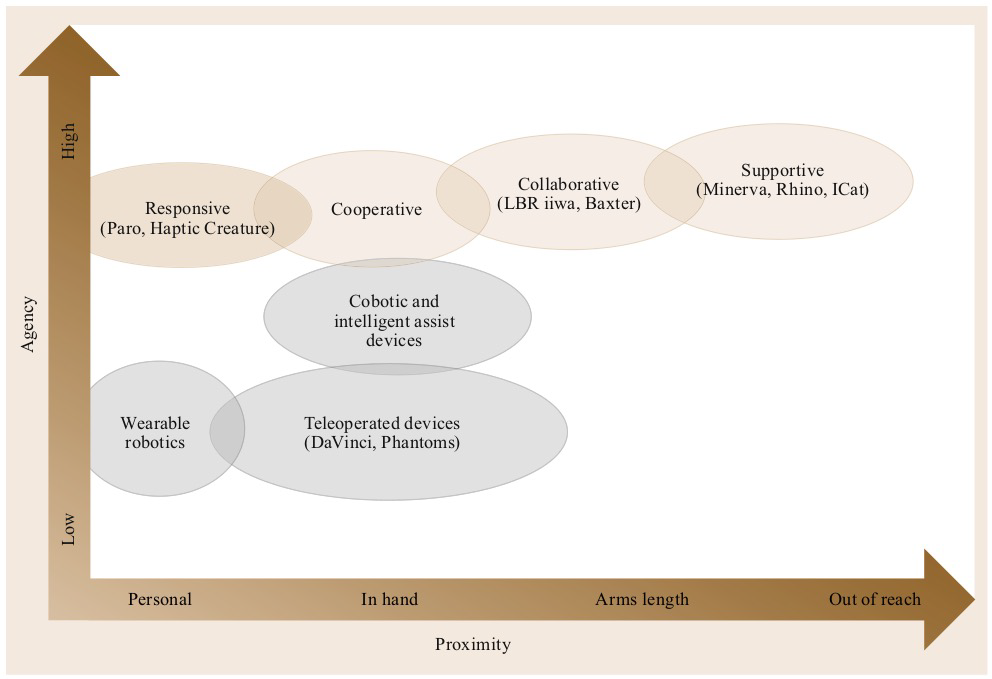
\includegraphics[width=\linewidth]{imgs/hri_interaction_types.png}
  \caption{Different types of human-robot interaction based on agency and proximity [Siciliano2016].}
\end{figure}

\hfill

\subsection{Supportive interaction}

In supportive interaction, the robot does not play the main role in the task. Instead, it supports the human operator by providing tools, materials, or information to enhance performance or help achieve specific objectives.

Examples include:
\begin{itemize}
  \item Museum guides
  \item Assistive robots
\end{itemize}

Safety is typically not an issue in this scenario because physical contact between the robot and the human rarely occurs. Furthermore, proximity control mechanisms are used to avoid unintended interactions.

\hfill

\subsection{Collaborative interaction}

In collaborative interaction, humans and robots work together on a task in a coordinated but separate manner. Each participant performs the part of the task that best suits their specific skills.

Some types of interaction are foreseen, such as:
\begin{itemize}
  \item Tool handover between robot and human
  \item Physical contact used intentionally to change the robot’s mode of operation (e.g., pushing the robot)
\end{itemize}

\hfill

\subsection{Cooperative interaction}

Cooperative interaction involves the human and robot jointly manipulating an object, leading to inevitable physical contact.

In this mode, both human and robot operate in direct contact—or through a shared object—with continuous shared control of the task execution.

This form of interaction is employed in scenarios such as:
\begin{itemize}
  \item Kinesthetic teaching
  \item Lifting and transportation
  \item Collaborative assembly
  \item Rehabilitation
\end{itemize}

\hfill

\subsection{Industrial Robotics: market data}

The annual installations of industrial robots have grown significantly over the last decade, reaching over 500,000 units worldwide in 2021.

\begin{figure}[H]
  \centering
  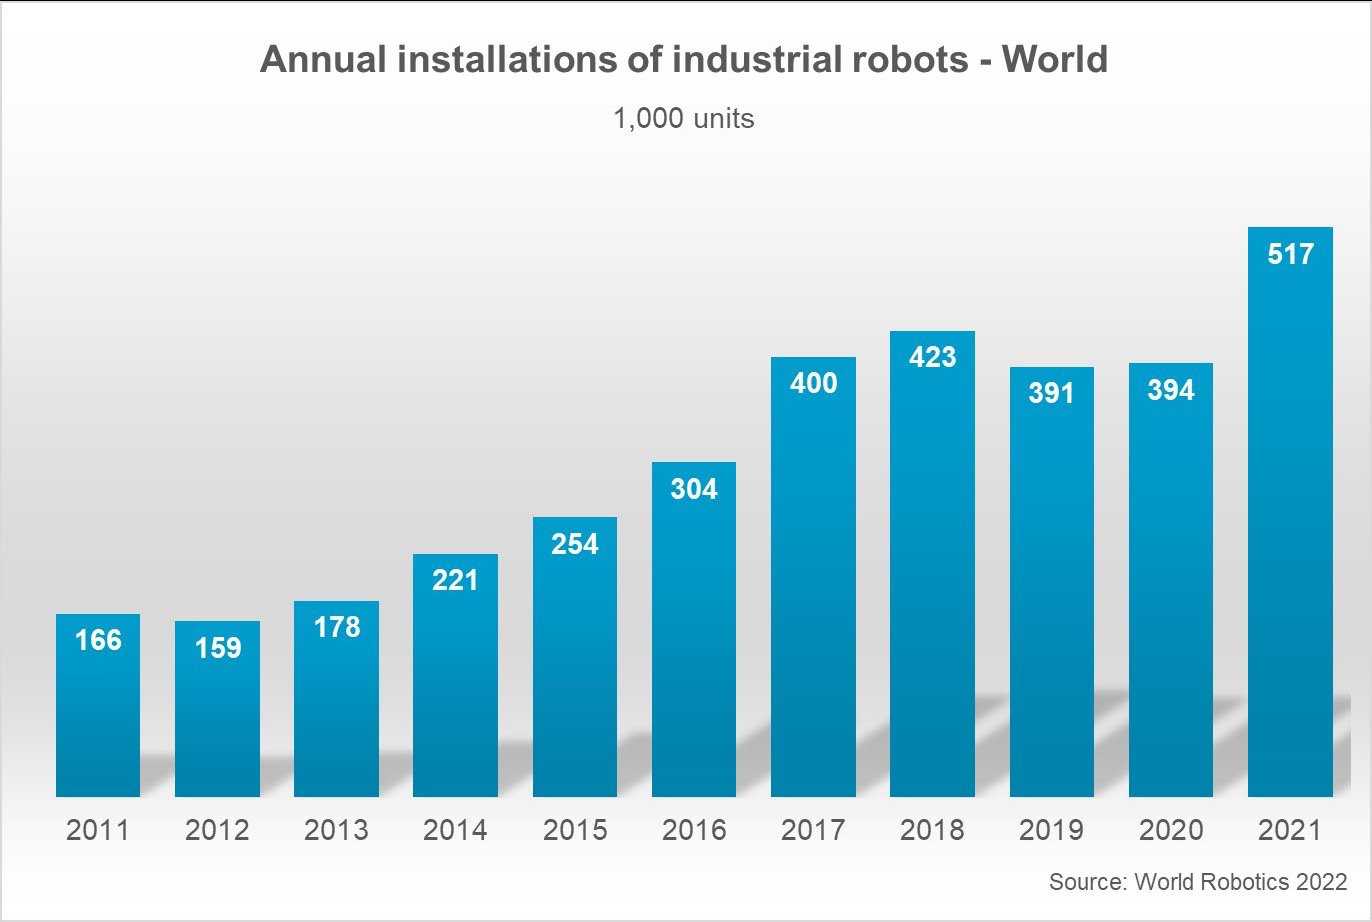
\includegraphics[width=0.85\linewidth]{imgs/industrial_robotics_world_installations.png}
  \caption{Annual installations of industrial robots worldwide (Source: World Robotics 2022).}
\end{figure}

The most demanding industries for industrial robots are electronics, automotive, and metal/machinery.

\begin{figure}[H]
  \centering
  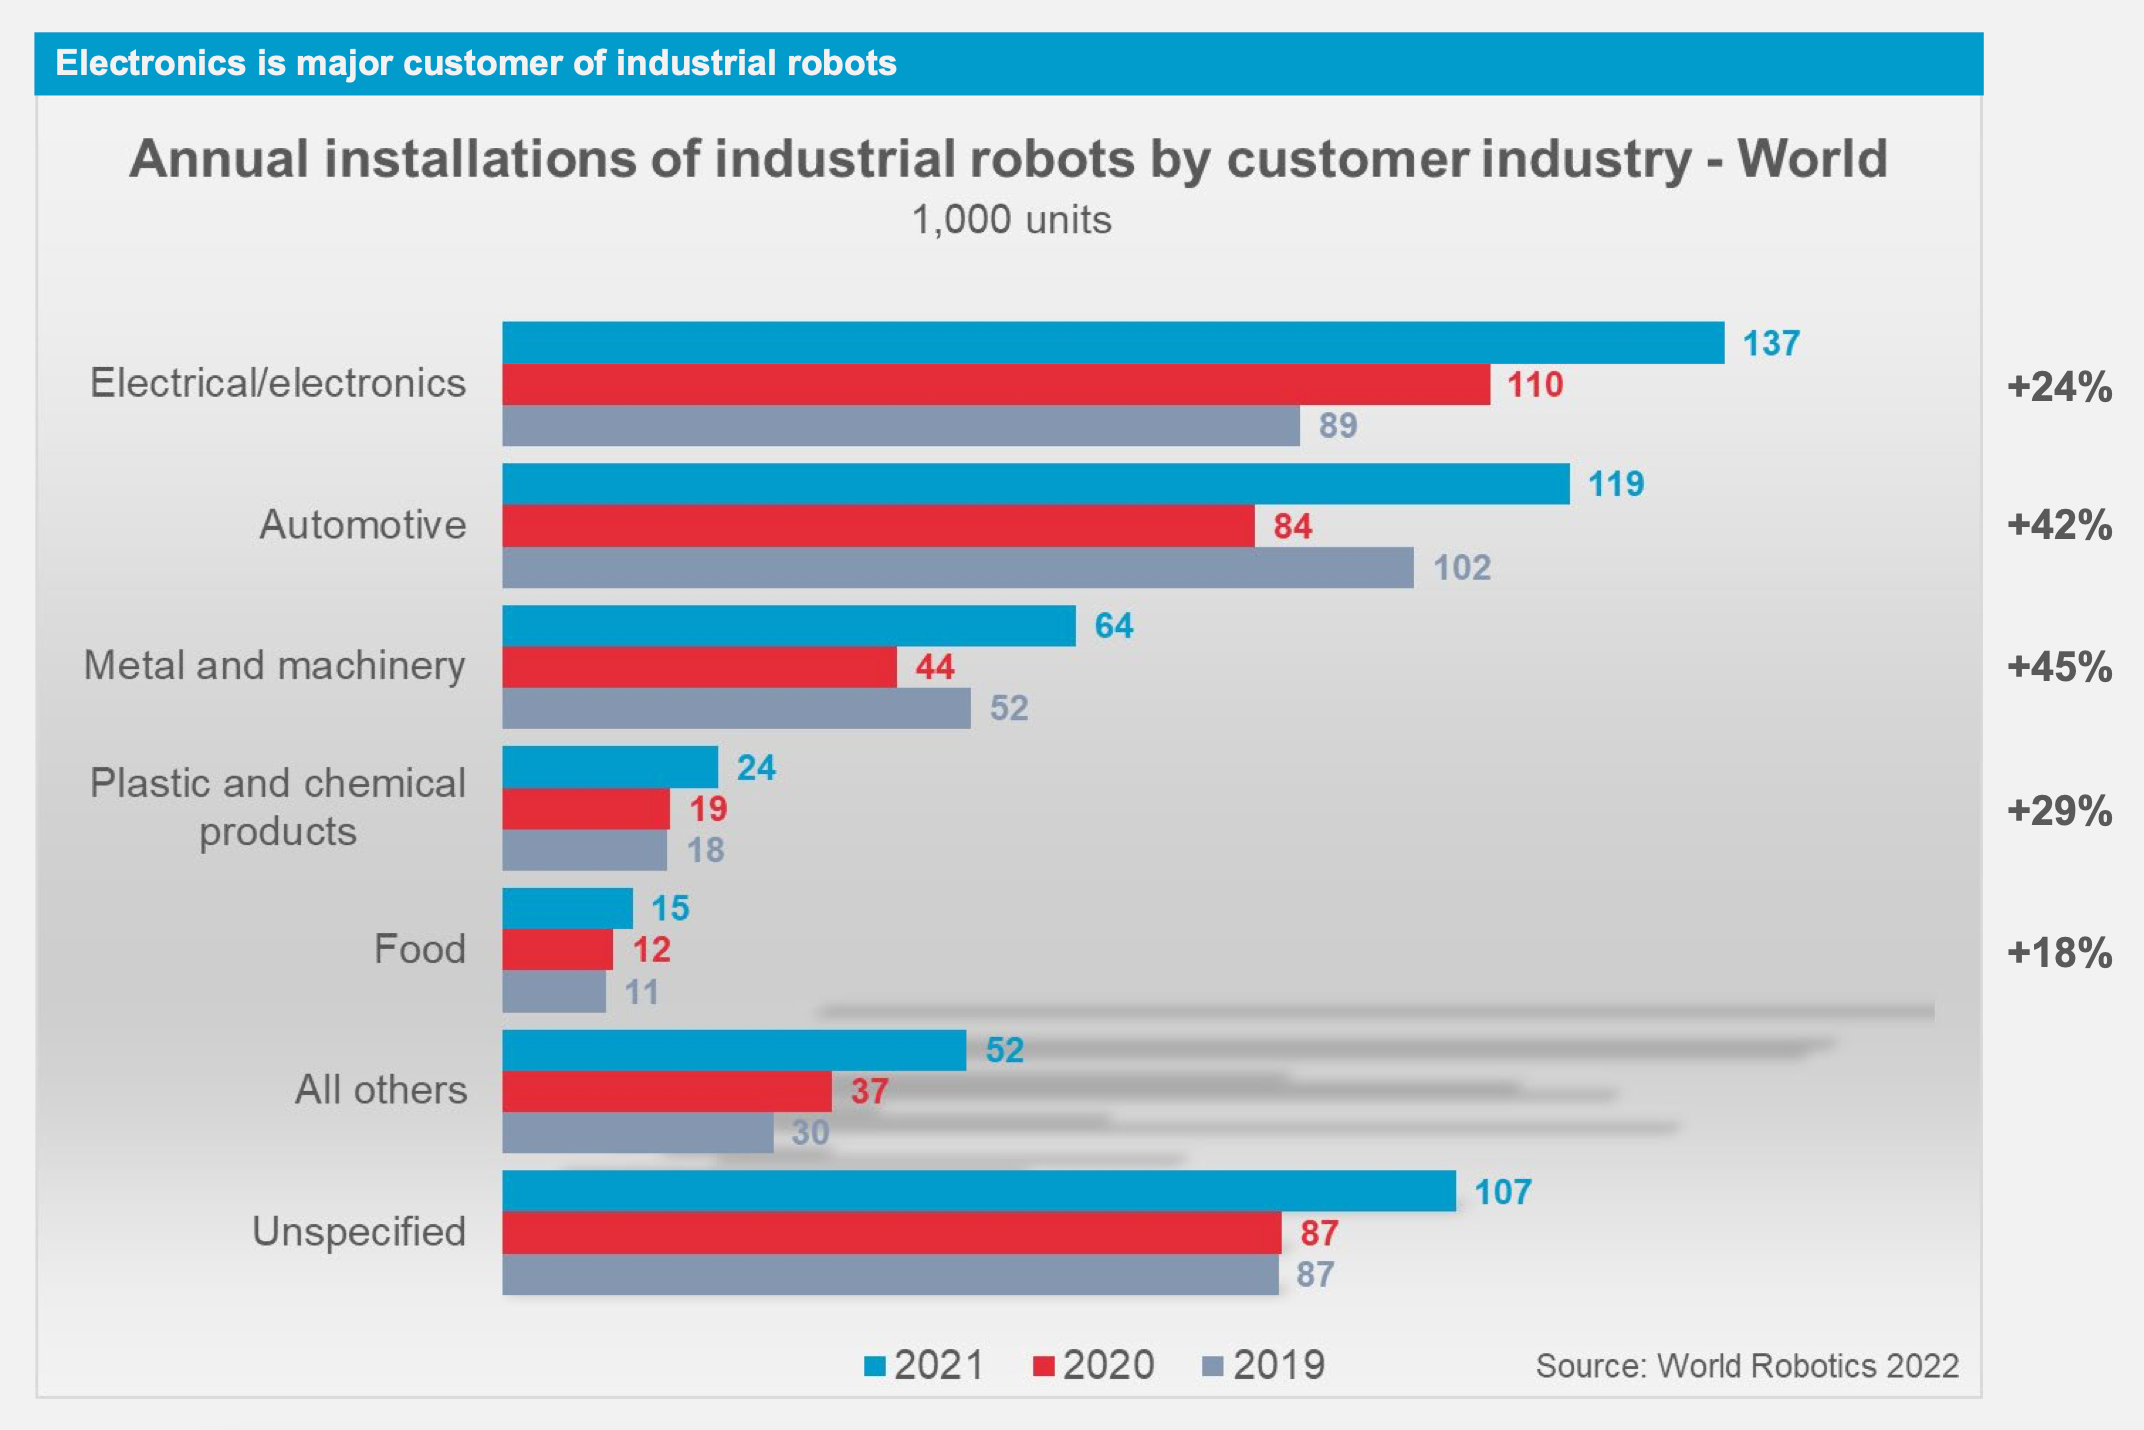
\includegraphics[width=0.85\linewidth]{imgs/industrial_robotics_by_industry.png}
  \caption{Robot installations by industry sector (Source: World Robotics 2022).}
\end{figure}

\hfill

\subsection{Industrial vs Collaborative Robotics}

Collaborative robots are still a small portion of total installations but are steadily growing, reaching 39,000 units in 2021 with a 50\% increase compared to the previous year.

\begin{figure}[H]
  \centering
  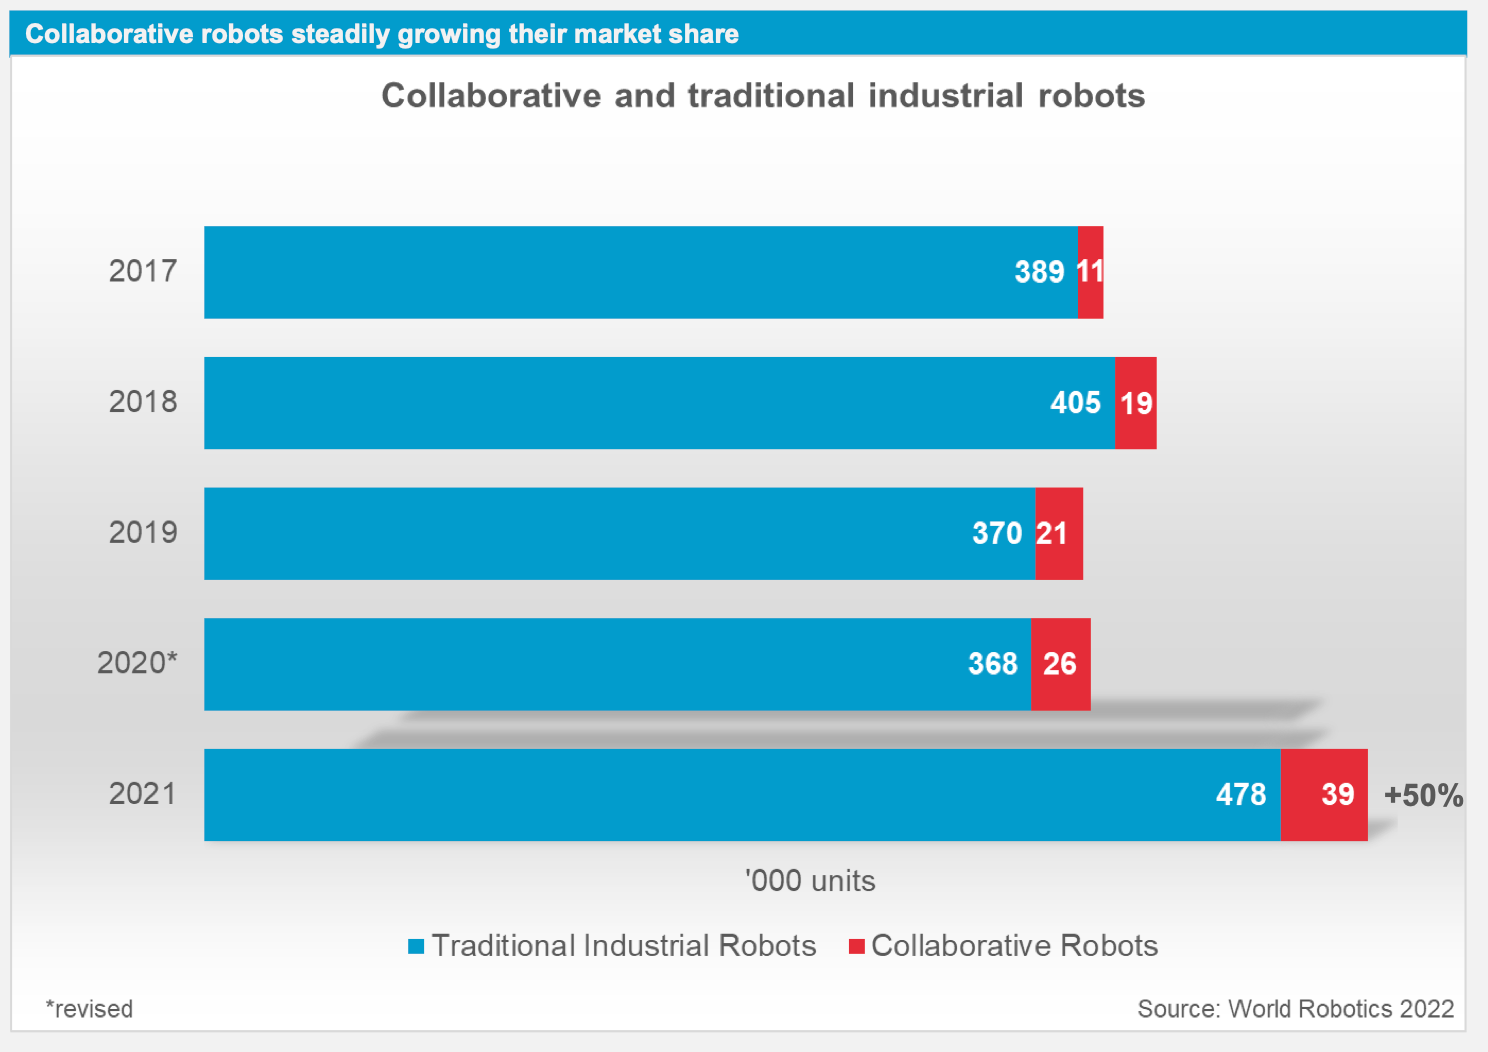
\includegraphics[width=0.85\linewidth]{imgs/industrial_vs_collaborative_robots.png}
  \caption{Comparison between industrial and collaborative robot installations (Source: World Robotics 2022).}
\end{figure}

\hfill

\subsection{Robotics in the World}

China leads the global robotics market by far, followed by Japan, the United States, and South Korea. Italy is in the top 5, with a significant growth rate of +65\%.

\begin{figure}[H]
  \centering
  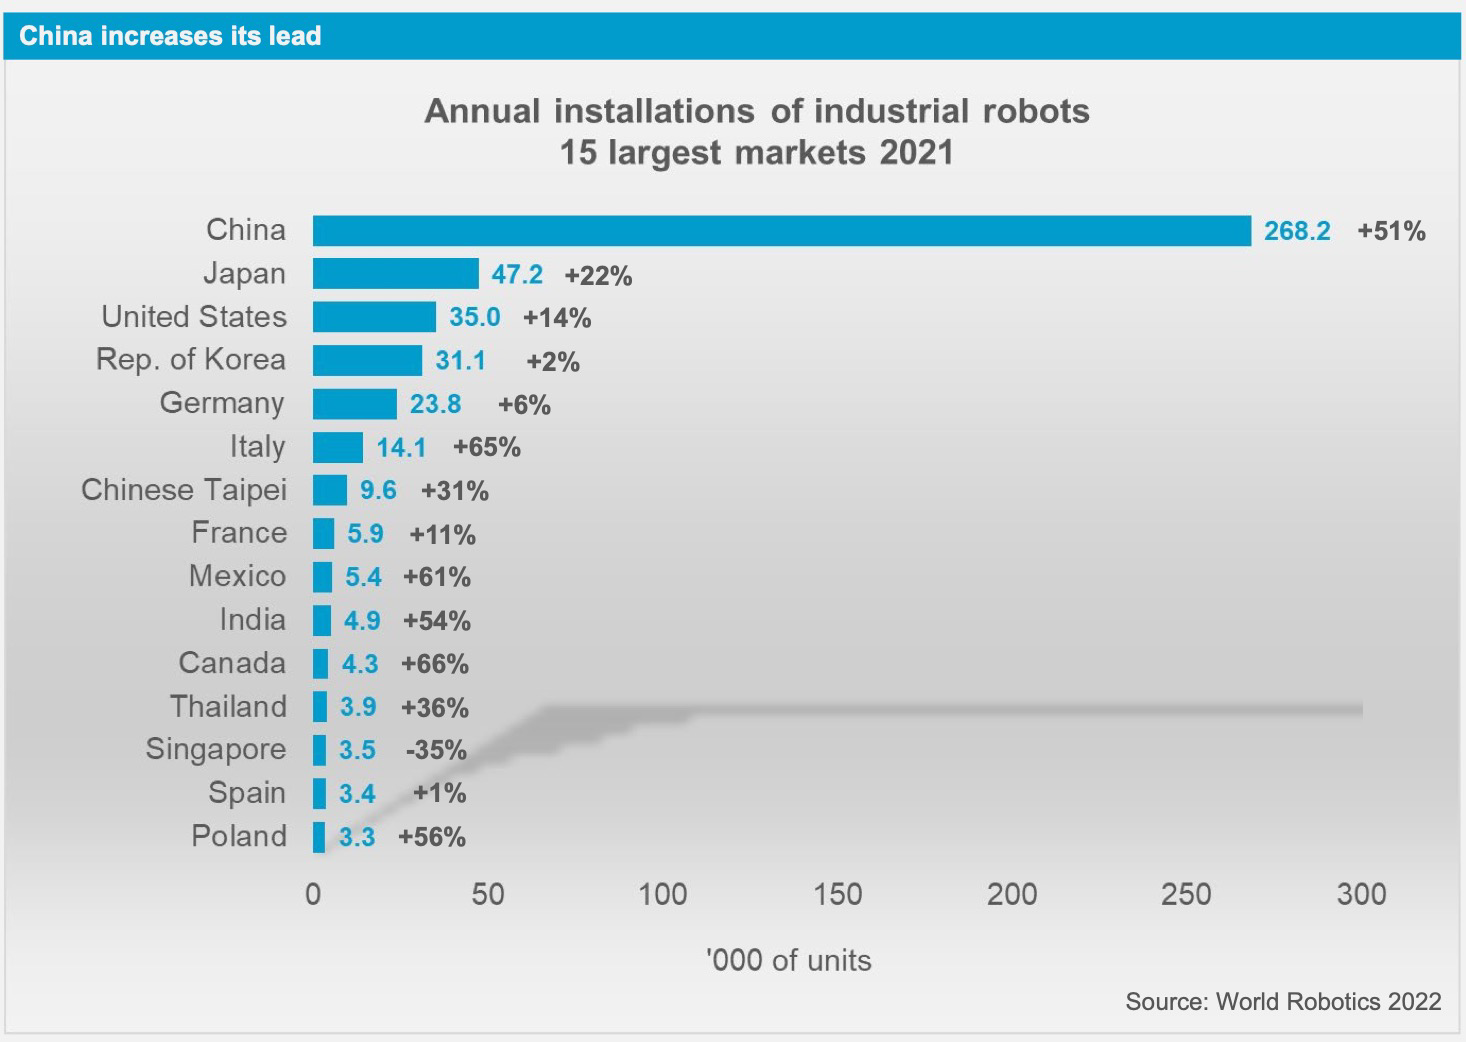
\includegraphics[width=0.85\linewidth]{imgs/robotics_by_country.png}
  \caption{Top 15 countries for robot installations in 2021 (Source: World Robotics 2022).}
\end{figure}

\newpage